\documentclass[10pt]{article}
% Layout of a NeurIPS/ICML submission: single column, 10pt Times, 5.5in x 9in text block.
% Swapping in a venue's style file is a one-line change.
\usepackage[letterpaper,textwidth=5.5in,textheight=9in,top=1in,headsep=0pt,headheight=0pt,footskip=30pt]{geometry}
\usepackage[T1]{fontenc}
\usepackage{times}
\usepackage{microtype}
\usepackage{amsmath,amssymb,amsthm,mathtools}
\usepackage{thm-restate}
\usepackage{booktabs,array}
\usepackage{placeins}
\usepackage{graphicx}
\usepackage[font=small,labelfont=bf]{caption}
\usepackage{tikz}
\usepackage{framed}
\usepackage{needspace}
\usetikzlibrary{positioning,arrows.meta,calc}
\usepackage[round,sort]{natbib}
\renewcommand{\bibfont}{\small\raggedright}
\renewcommand{\bibsection}{\section*{References}\addcontentsline{toc}{section}{References}}
\usepackage[colorlinks,linkcolor=blue!45!black,citecolor=blue!45!black,urlcolor=blue!45!black]{hyperref}
\usepackage[capitalise,noabbrev,nameinlink]{cleveref}
\usepackage{enumitem}
\setlist{nosep,leftmargin=1.4em}
\setlength{\textfloatsep}{10pt plus 2pt minus 2pt}
\renewcommand{\topfraction}{0.85}
\renewcommand{\textfraction}{0.1}

% TeX Live 2026 (LaTeX 2026-06-01) makes a theorem that shares a counter an alias of it (\newcounteralias),
% and thmtools, loaded by thm-restate, would make the same alias again, an error. Leave the alias to LaTeX;
% on older TeX Live, without \newcounteralias, nothing changes.
\makeatletter
\@ifundefined{newcounteralias}{}{%
  \renewcommand\thmt@autorefsetup{\@xa\def\csname\thmt@envname autorefname\@xa\endcsname\@xa{\thmt@thmname}}%
}
\makeatother
\newtheorem{theorem}{Theorem}[section]
\newtheorem{proposition}[theorem]{Proposition}
\newtheorem{corollary}[theorem]{Corollary}
\newtheorem{lemma}[theorem]{Lemma}
\newtheorem{conjecture}{Conjecture}
\theoremstyle{definition}
\newtheorem{definition}[theorem]{Definition}
\newtheorem*{definition*}{Definition}
\theoremstyle{remark}
\newtheorem{remark}[theorem]{Remark}
\crefname{equation}{}{}
\crefname{conjecture}{Conjecture}{Conjectures}
\Crefname{conjecture}{Conjecture}{Conjectures}

\newcommand{\R}{\mathbb{R}}
\newcommand{\Wread}{W_{\mathrm{read}}}
\newcommand{\Wwrite}{W_{\mathrm{write}}}
\newcommand{\dm}{d_{\mathrm{model}}}
\newcommand{\GL}{\mathrm{GL}}
\newcommand{\Ort}{\mathrm{O}}
\newcommand{\CO}{\mathrm{CO}}
\newcommand{\Aff}{\mathrm{Aff}}
% The Frechet derivative, upright to set it apart from the readout D.
\newcommand{\Der}{\mathrm{D}}
\newcommand{\G}{\mathcal{G}}
\newcommand{\norm}[1]{\lVert #1\rVert}
\newcommand{\para}[1]{\smallskip\noindent\textbf{#1}\hspace{0.5em}}
% The one-sentence summary at the start of a main section.
\newcommand{\takeaway}[1]{\noindent\textit{#1}\par\smallskip}
% A link from a result in the main text to its proof in Appendix A.
% A link target at a part of a statement, and references that link name, number and part to it.
\newcommand{\ptlabel}[1]{\phantomsection\label{#1}}
\DeclareRobustCommand{\cpref}[2]{\hyperref[#1:#2]{\cref*{#1}(#2)}}
\DeclareRobustCommand{\Cpref}[2]{\hyperref[#1:#2]{\Cref*{#1}(#2)}}
\DeclareRobustCommand{\rpref}[2]{\hyperref[#1:#2]{\ref*{#1}(#2)}}
\DeclareRobustCommand{\ptlink}[2]{\hyperref[#1:#2]{(#2)}}
\newcommand{\proofin}[1]{\par\vspace{-0.4\baselineskip}\noindent\hfill{\small\itshape Proof in \cref{#1}.}\par\smallskip}
% A main-text result that is a special case of, or follows from, a result in the appendix.
\newcommand{\specialof}[2]{\par\vspace{-0.4\baselineskip}\noindent\hfill{\small\itshape A special case of \cref{#1}, proved in \cref{#2}.}\par\smallskip}
\newcommand{\followsfrom}[2]{\par\vspace{-0.4\baselineskip}\noindent\hfill{\small\itshape Follows from \cref{#1}, proved in \cref{#2}.}\par\smallskip}
% A part of a statement: a link target (if a label is given), a bold number in parentheses and an optional bold name.
\newcommand{\stpart}[3]{\ifx\relax#1\relax\else\ptlabel{#1:#2}\fi{\upshape\bfseries\boldmath(#2)\ifx\relax#3\relax\else\ #3.\fi}}
% A lemma and its proof inside another proof: indented, with a thin gray rule on the left.

\title{\Large\bfseries\boldmath How Many Hidden Units Is a Skip Connection Worth?}

\newif\ifanon \anonfalse
\ifanon
\author{Anonymous authors}
\else
\author{Antonij Mijoski$^{*}$\\ IRMA, Universit\'e de Strasbourg\\ {\small\texttt{antonij.mijoski@unistra.fr}}\\ {\small\texttt{antonijmijo@gmail.com}}
\and Marko Karbevski$^{*\dagger}$\\ In Simplicity Technologies\\ {\small\texttt{markokarbevski@insimplicity.tech}}\\ {\small\texttt{markokarbevski@gmail.com}}}
\fi
\date{}

\begin{document}
\maketitle
\suppressfloats[t]
\ifanon\else
{\renewcommand{\thefootnote}{$*$}%
\footnotetext{\emph{Author contributions.} Marko Karbevski (MK) conceived and led the study. Antonij Mijoski (AM) proved the absorption result for a single ReLU block (\cpref{thm:relugelu}{i}, \cref{thm:f3}), the difficult case, paving the way forward. MK extended the tools to GELU (\cref{thm:f4}), proved the cases of ReLU$^2$ and of the gated (GLU) variants (\cref{thm:homgated,thm:homgatednet}) and the results at depth (\cref{thm:relufirst,prop:extraunits}), and worked on the symmetry breaking across layers and its counting, the parameter counts at model scale and the applications. Both authors worked on the experiments and on the writing. All of MK's work on the results, the proofs and the experiments was done with AI assistants.}}
{\renewcommand{\thefootnote}{$\dagger$}\footnotetext{Corresponding author.}}
\fi
\vspace{-1.5em}

\begin{abstract}
Residual networks add the input of every block to its output, $x + B(x)$, and skipless networks can now be trained to match them. Whether the skip lets a block compute functions that it cannot compute alone has had no exact answer. Here we show that a skip connection is worth exactly $\dm$ hidden ReLU or GELU units, and more than any number of ReLU$^2$, ReGLU, SwiGLU, GeGLU or $\tanh$ units or attention heads. With an embedding and a readout, residual networks of gated, homogeneous or $\tanh$ blocks equal no skipless network, a skipless ReLU network needs $2\dm$ units in its first block to equal almost any residual one, and under RMSNorm with $\varepsilon = 0$ almost no residual network is skipless at any width. Yet every skipless network is a limit of residual networks of the same widths. These prices tell exactly when a residual model can be rewritten without its skips.
\end{abstract}

\section{Introduction}\label{sec:intro}

Almost every deep network trained today adds the input of a block to its output. A residual block computes $x + B(x)$ \citep{he2016resnet}, and transformers stack such blocks \citep{vaswani2017attention}. The usual reason is training: the sum gives the gradient a short path through the network, and it makes the identity map easy to express \citep{veit2016ensembles,hardt2017identity}.

Skipless networks now train too. \citet{he2024simplifying} remove the skips of transformer blocks without losing training speed, and \citet{ji2026cutting} train a skipless ViT-B on ImageNet that outperforms the residual one. So does a skip only help training, or does it also let a block compute functions that it cannot compute alone?

We answer this question exactly. Take an MLP block $B$ with $N$ hidden units. Is the residual block $x \mapsto x + B(x)$ also a block of the same kind without a skip, with $N$ hidden units or with more? If it is, the skip costs some hidden units and nothing else. If it is not, no width can replace it.

\para{The answer depends on the activation, and it is sharp.}
\begin{itemize}
\item ReLU and GELU blocks pay exactly $\dm$ units. With $\dm$ more units a block absorbs its skip, because $\sigma(z) - \sigma(-z) = z$ for both activations; for almost every block, fewer units do not suffice (\cref{thm:relugelu}).
\item ReLU$^2$, ReGLU, SwiGLU, GeGLU and $\tanh$ blocks cannot pay at any width (\cref{thm:homgated}).
\item Attention blocks cannot pay with any number of heads (\cref{thm:attention}).
\end{itemize}

\para{Three one-line reasons.} Follow the input along a ray, $x = tu$ with $t > 0$. The skip grows like $t$. A ReLU$^2$ block grows like $t^2$, a gated block starts at order $t^2$ near the origin, and a $\tanh$ block stays bounded, so none of them can produce the linear term (\cref{fig:reasons}). Attention mixes the tokens of a sequence, while a skip leaves each token where it is.

\para{Networks.} The picture survives in networks with an embedding and a readout, with one twist for ReLU: a skipless ReLU network needs $2\dm$ units in its first block to equal almost any residual one (\cref{thm:relufirst}). Under RMSNorm with $\varepsilon = 0$, a skipless network forgets the length of its input and the skip keeps it, so no width helps (\cref{prop:epszero}).

\para{Exact, yet approximable.} Every skipless network is a limit of residual networks of the same widths (\cref{prop:limits}). So the skip adds functions that skipless networks cannot compute exactly, while residual networks can still approach every skipless one. \Cref{tab:results} collects the results; \cref{sec:setup} fixes the setting, \cref{sec:oneblock} treats one block, \cref{sec:networks} networks and \cref{sec:limits} limits. Proofs are in the appendix.

\begin{table}[t]
\centering\small
\renewcommand{\arraystretch}{1.12}
\setlength{\tabcolsep}{3pt}
\newcommand{\cell}[1]{\begin{tabular}[c]{@{}c@{}}#1\end{tabular}}
\newcommand{\rtag}[3]{{\footnotesize\if\relax\detokenize{#3}\relax\hyperref[#2]{#1~\ref*{#2}}\else\hyperref[#2:#3]{#1~\ref*{#2}(#3)}\fi}}
\newcommand{\res}[4]{\cell{#1\\ \rtag{#2}{#3}{#4}}}
\makebox[\linewidth][c]{\begin{tabular}{|l|c|c|c|c|c|c|}
\hline
\textbf{Proven} & \textbf{ReLU} & \textbf{GELU} & $\boldsymbol{\tanh}$ & \cell{\textbf{ReLU$\boldsymbol{^2}$,}\\ \textbf{ReGLU}} & \cell{\textbf{SwiGLU,}\\ \textbf{GeGLU}} & \textbf{Attention} \\
\hline
one block, same width & \multicolumn{2}{c|}{\res{measure zero}{Thm.}{thm:relugelu}{i}} & \multicolumn{3}{c|}{\res{never}{Thm.}{thm:homgated}{}} & \res{never}{Thm.}{thm:attention}{i} \\
\hline
one block, more units & \multicolumn{2}{c|}{\res{exactly $\dm$ more}{Thm.}{thm:relugelu}{ii}} & \multicolumn{3}{c|}{\res{no number}{Thm.}{thm:homgated}{}} & \res{no number of heads}{Thm.}{thm:attention}{i} \\
\hline
networks, $L = 1$ & \multicolumn{2}{c|}{\res{measure zero}{Thm.}{thm:relugelu}{i}} & \res{never}{Thm.}{thm:homgatednet}{iii} & \multicolumn{2}{c|}{\res{never}{Thm.}{thm:homgatednet}{ii}} & \res{never}{Thm.}{thm:attention}{ii} \\
\hline
networks, $L \ge 2$ & \cell{measure zero if the\\ first block has fewer\\ than $2\dm$ units\\ \rtag{Thm.}{thm:relufirst}{}} & -- & \res{never}{Thm.}{thm:homgatednet}{iii} & \multicolumn{2}{c|}{\res{never}{Thm.}{thm:homgatednet}{ii}} & -- \\
\hline
networks, more units & \multicolumn{2}{c|}{\res{$\dm$ more per block suffice}{Prop.}{prop:extraunits}{}} & \res{no number}{Thm.}{thm:homgatednet}{iii} & \multicolumn{2}{c|}{\res{no number}{Thm.}{thm:homgatednet}{ii}} & -- \\
\hline
with pre-RMSNorm, $\varepsilon > 0$ & -- & -- & -- & \multicolumn{2}{c|}{\res{never}{Thm.}{thm:homgatednet}{ii}} & -- \\
\hline
with pre-RMSNorm, $\varepsilon = 0$ & \multicolumn{6}{c|}{\res{measure zero, at any width}{Prop.}{prop:epszero}{iii}} \\
\hline
skipless are limits of residual & \multicolumn{6}{c|}{\cell{yes, at the same widths \rtag{Prop.}{prop:limits}{i}; with pre-RMSNorm, $\varepsilon = 0$, \rtag{Prop.}{prop:limits}{ii}}} \\
\hline
\end{tabular}}
\caption{Can a skipless network equal a residual one? Never: for no weights and no width. Measure zero: only for weights in a set of measure zero. A dash: not settled here (\cref{sec:conclusion}). Networks have an embedding $E$ and a readout $D$ with $ED \neq 0$, and no biases.}
\label{tab:results}
\end{table}

\section{Setup}\label{sec:setup}
\takeaway{One equation states the question: can a block absorb a linear term?}

\para{Blocks.} A hidden state is a matrix $h \in \R^{T\times\dm}$ whose rows are the $T$ tokens of a sequence. An MLP block acts on each token separately. On a row $x \in \R^{1\times\dm}$ it computes
\begin{equation}\label{eq:mlp}
B_\theta(x) = f(x\Wread)\,\Wwrite, \qquad \theta = (\Wread, \Wwrite),
\end{equation}
with a read $\Wread$ and a write $\Wwrite$. In a vanilla block with $N$ hidden units, $\Wread \in \R^{\dm\times N}$, $\Wwrite \in \R^{N\times\dm}$, and $f$ applies an activation $\sigma$ to each unit: ReLU, GELU, $\tanh$ or ReLU$^2$, $\sigma(z) = \max(z,0)^2$. In a gated block the read has two halves, $\Wread = [\,W_{\mathrm g} \mid W_{\mathrm v}\,]$, and unit $i$ computes $\sigma\big((xW_{\mathrm g})_i\big)\,(xW_{\mathrm v})_i$, with $\sigma$ the ReLU in ReGLU, SiLU in SwiGLU and GELU in GeGLU \citep{shazeer2020glu}. Attention blocks follow in \cref{sec:attention}.

\para{The question as an equation.} A skip adds $x$ to the output of a block. More generally, can a block absorb a linear term $xM$, for a $\dm\times\dm$ matrix $M \neq 0$? We look for parameters $\theta'$ of a block with the same activation, and of any width, such that
\begin{equation}\label{eq:absorbask}
xM + B_\theta(x) = B_{\theta'}(x) \qquad\text{for all } x \in \R^{1\times\dm}.
\end{equation}
The skip is $M = I$. Other matrices cover learned linear skips and, below, networks.

\para{Networks.} A network maps an input $x$ to $h_0 = xE$ with an embedding $E$, passes it through $L$ blocks, and returns $y = h_LD$ with a readout $D$. A \emph{skipless} network has $h_\ell = B_\ell(h_{\ell-1})$, and a \emph{residual} network has $h_\ell = h_{\ell-1} + B_\ell(h_{\ell-1})$. In a \emph{pre-RMSNorm} network every block and the readout read the normalized state $N(h)$, which divides each row of $h$ by $\sqrt{\norm{h}^2/\dm + \varepsilon}$, where $\norm{h}$ is the norm of that row.

\para{Scope.} For simplicity, networks have no biases, every block has at least $\dm$ hidden units, all MLP blocks of a network are of one kind, all attention blocks have the same number of heads, and inputs and outputs have dimension at least $\dm \ge 2$. Most results hold more generally, and the appendix states them so. \emph{Almost every} choice of weights means every choice outside a set of Lebesgue measure zero.

\section{One block}\label{sec:oneblock}
\takeaway{A ReLU or GELU block pays exactly $\dm$ units for its skip. The other blocks cannot pay at any width.}

\subsection{ReLU and GELU blocks pay \texorpdfstring{$\dm$}{d\_model} units}\label{sec:relugelu}

Both activations satisfy
\begin{equation}\label{eq:odd}
\sigma(z) - \sigma(-z) = z,
\end{equation}
so a unit and its mirror image, the unit with the opposite read, add up to a linear term. This gives two ways to absorb $xM$.

\emph{With more units.} Let unit $i$ have read $w_i$ and write $a_i$. A new unit with read $-w_i$ and write $-b$, together with the write $a_i + b$ for unit $i$, adds $(xw_i)\,b$ to the block, by \eqref{eq:odd}. So each new unit adds one rank-one term, and $\dm$ new units, mirroring $\dm$ units whose reads span $\R^{\dm}$, add any $xM$.

\emph{At the same width.} Flipping the read of unit $i$ to $-w_i$ changes the block by $-(xw_i)\,a_i$. So a block of the same width absorbs $xM$ if some set $S$ of units has $\Wread[{:},S]\,\Wwrite[S,{:}] = -M$, where $\Wread[{:},S]$ and $\Wwrite[S,{:}]$ keep the columns and rows of the units in $S$.

The theorem says that these are the only ways. A block is \emph{nondegenerate} if the columns of $\Wread$ are nonzero and pairwise non-collinear and the rows of $\Wwrite$ are nonzero.

\begin{restatable}[ReLU and GELU blocks]{theorem}{thmAbsorbReLU}\label{thm:relugelu}
Let $\sigma$ be ReLU or GELU.\\
\stpart{thm:relugelu}{i}{} If $B_\theta$ is nondegenerate, a block $B_{\theta'}$ of the same width satisfies \eqref{eq:absorbask} if and only if some set $S$ of hidden units has $\Wread[{:},S]\,\Wwrite[S,{:}] = -M$; for generic $\theta$ there is none.\\
\stpart{thm:relugelu}{ii}{} If $M$ is invertible and $\Wread$ has rank $\dm$, a block $B_{\theta'}$ with $\dm$ more hidden units satisfies \eqref{eq:absorbask}, and for generic $\theta$ none with fewer does.
\end{restatable}
\proofin{app:absorb}

For generic weights no set of units has the required product: there are finitely many sets, and each gives one matrix. So the skip, $M = I$, costs exactly $\dm$ units. The proof matches the units of the two blocks. The even part of the activation, $\big(\sigma(z) + \sigma(-z)\big)/2$, determines the hidden units of the absorbing block up to sign and scale, through the kinks of $\lvert z\rvert$ for ReLU and through the linear independence of ridge functions for GELU; the odd part, $z/2$, turns each sign flip into a linear term, as \citet[Section~3]{petzka2020symmetries} show for two-layer ReLU networks with one output. Each extra unit then adds at most one rank-one term, and $M = I$ has rank $\dm$.

\para{Networks of one block.} A network of one block computes $x \mapsto xED + f(xE\Wread)\,\Wwrite D$. \Cref{thm:relugelu} applies with the reads $E\Wread$, the writes $\Wwrite D$ and $M = ED$, so a skipless network of the same width equals it only for weights in a set of measure zero.

\subsection{Blocks that never absorb a skip}\label{sec:never}

\begin{figure}[t]
\centering
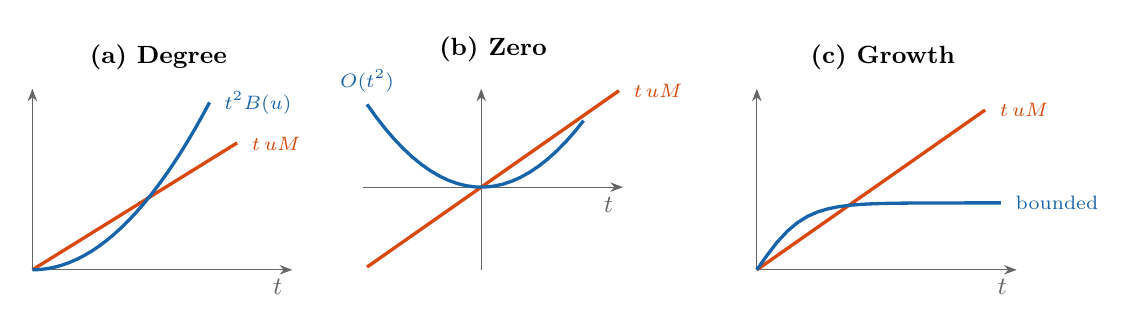
\begin{tikzpicture}[x=1cm,y=1cm,font=\small]
\tikzset{ax/.style={-{Stealth[length=1.6mm]},black!60}, skip/.style={very thick,color={rgb,255:red,217;green,72;blue,15}}, blk/.style={very thick,color={rgb,255:red,24;green,100;blue,171}}, ttl/.style={font=\bfseries\small}}
\begin{scope}
\draw[ax] (0,0) -- (3.3,0) node[below left] {$t$};
\draw[ax] (0,0) -- (0,2.3);
\draw[skip, domain=0:2.6] plot (\x, {0.62*\x});
\draw[blk, domain=0:2.25] plot (\x, {0.42*\x*\x});
\node[skip, anchor=west, font=\scriptsize] at (2.65,1.6) {$t\,uM$};
\node[blk, anchor=west, font=\scriptsize] at (2.3,2.12) {$t^2 B(u)$};
\node[ttl] at (1.6,2.7) {(a) Degree};
\end{scope}
\begin{scope}[xshift=5.7cm, yshift=1.05cm]
\draw[ax] (-1.5,0) -- (1.8,0) node[below left] {$t$};
\draw[ax] (0,-1.05) -- (0,1.25);
\draw[skip, domain=-1.45:1.75] plot (\x, {0.7*\x});
\draw[blk, domain=-1.45:1.3] plot (\x, {0.5*\x*\x});
\node[skip, anchor=west, font=\scriptsize] at (1.8,1.22) {$t\,uM$};
\node[blk, anchor=south, font=\scriptsize] at (-1.45,1.07) {$O(t^2)$};
\node[ttl] at (0.15,1.75) {(b) Zero};
\end{scope}
\begin{scope}[xshift=9.2cm]
\draw[ax] (0,0) -- (3.3,0) node[below left] {$t$};
\draw[ax] (0,0) -- (0,2.3);
\draw[skip, domain=0:2.9] plot (\x, {0.7*\x});
\draw[blk, domain=0:3.1] plot (\x, {0.85*tanh(1.7*\x)});
\node[skip, anchor=west, font=\scriptsize] at (2.95,2.03) {$t\,uM$};
\node[blk, anchor=west, font=\scriptsize] at (3.15,0.85) {bounded};
\node[ttl] at (1.6,2.7) {(c) Growth};
\end{scope}
\end{tikzpicture}
\caption{Why no width absorbs the skip. Along a ray $x = tu$ the skip grows like $t$. (a) A homogeneous block of degree $2$ grows like $t^2$. (b) A gated block is of order $t^2$ near $t = 0$. (c) A $\tanh$ block stays bounded.}
\label{fig:reasons}
\end{figure}

\begin{restatable}[Blocks that never absorb a skip]{theorem}{thmAbsorbHom}\label{thm:homgated}
Let the block be positively homogeneous of degree $k \neq 1$, as ReLU$^2$ and ReGLU blocks are, or gated with a gate that is differentiable at $0$ and vanishes there, as SwiGLU and GeGLU blocks are, or a $\tanh$ block. No block $B_{\theta'}$ of any width satisfies \eqref{eq:absorbask}.
\end{restatable}
\proofin{app:absorb}

The three cases of \cref{fig:reasons} are three one-line proofs. A homogeneous block satisfies $B(tu) = t^kB(u)$ for $t > 0$, so along a ray \eqref{eq:absorbask} reads $t\,uM = t^k\big(B'(u) - B(u)\big)$, which forces $uM = 0$ for every $u$ when $k \neq 1$. A gate that vanishes at $0$ makes every unit of order $t^2$ near the origin, so both blocks have derivative $0$ there, while $xM$ has derivative $M$. A $\tanh$ block is bounded, and $xM$ is not. A linear block, by contrast, absorbs any skip: $xM + xA = x(M + A)$.

\subsection{Attention blocks never absorb a skip}\label{sec:attention}

Attention mixes tokens, and a skip keeps each token where it is. Two inputs make this precise. If all tokens are equal, mixing changes nothing, so the heads must reproduce the skip. If one token is zero, its query is zero, so attention gives it an equal mix of all tokens. The skip gives it zero.

An \emph{attention block} with parameters $\theta = (W_{Q,i}, W_{K,i}, W_{V,i}, W_{O,i})_{i=1}^{H}$ maps $h \in \R^{T\times\dm}$, whose rows are the $T \ge 2$ tokens, to
\begin{equation}\label{eq:attn}
B_\theta(h) = \sum_{i=1}^{H} P_{\Gamma_i}(h)\, h\, W_{V,i} W_{O,i}, \qquad P_\Gamma(h) = \mathrm{softmax}\big(h\, \Gamma h^\top\big), \qquad \Gamma_i = W_{Q,i} W_{K,i}^\top/\sqrt{d_h},
\end{equation}
where $W_{Q,i}, W_{K,i}, W_{V,i} \in \R^{\dm\times d_h}$ and $W_{O,i} \in \R^{d_h\times\dm}$. The softmax acts on each row of the $T\times T$ matrix of scores, with or without a causal mask, so each row of $P_\Gamma(h)$ is a probability vector. Head $i$ has the score matrix $\Gamma_i$ and the value--output product $W_{V,i}W_{O,i}$.

\begin{restatable}[Attention blocks]{theorem}{thmAttention}\label{thm:attention}
Let $\theta$ and $\theta'$ be parameters of attention blocks with any numbers and widths of heads, and let $M \neq 0$ be a $\dm\times\dm$ matrix.\\
\stpart{thm:attention}{i}{} For almost every $h \in \R^{T\times\dm}$, $hM + B_\theta(h) \neq B_{\theta'}(h)$.\\
\stpart{thm:attention}{ii}{} With an embedding $E$ and a readout $D$ with $ED \neq 0$, the residual network $x \mapsto \big(xE + B_\theta(xE)\big)D$ differs from every skipless network $x \mapsto B_{\theta'}(xE')D'$.
\end{restatable}
\specialof{thm:attentionfull}{app:attention}

The proof gives a gap: some input whose rows have norm at most $1$ has a row in which $hM + B_\theta(h)$ and $B_{\theta'}(h)$ differ by at least $\norm{M}/3$, where $\norm{M}$ is the spectral norm (\cpref{thm:attentionfull}{ii}). It uses only that each row of attention weights sums to $1$ and is uniform for a zero query, so it also holds with rotary position embeddings. Adding heads does not help, while $\dm$ more ReLU or GELU units absorb the skip of an MLP block.

\para{The softmaxes must match.} With three or more tokens there is a sharper reason: the heads of the two blocks must cancel each other exactly, and then nothing is left to produce $hM$. What tells heads apart is where their softmaxes have poles in the complex plane.

\begin{restatable}[The softmaxes must match]{proposition}{propMatch}\label{prop:match}
Let $T \ge 3$, let $\theta$ and $\theta'$ be parameters of attention blocks, and suppose that $hM + B_\theta(h) = B_{\theta'}(h)$ for all $h$ in a nonempty open set. Then $M = 0$, and for every matrix $\Gamma$, the heads with score matrix $\Gamma$ have the same sum of value--output products in $B_\theta$ as in $B_{\theta'}$.
\end{restatable}
\followsfrom{lem:heads}{app:attention}

With two tokens, heads can cancel: the softmax of two scores is the logistic function of their difference, and $1/(1 + e^{-z}) + 1/(1 + e^{z}) = 1$ makes two heads with opposite score matrices add up to a uniform head. A skip still cannot be absorbed when $T = 2$ (\cpref{thm:attention}{i}).

\section{Networks}\label{sec:networks}
\takeaway{With an embedding and a readout the picture survives. Gated, homogeneous and $\tanh$ networks never absorb their skips, and ReLU networks pay in their first block.}

Recall that a network embeds its input as $h_0 = xE$ and reads out $y = h_LD$, and that its skips add $h_{\ell-1}$ at every block.

\begin{restatable}[Networks that never absorb their skips]{theorem}{thmAbsorbHomNet}\label{thm:homgatednet}
\stpart{thm:homgatednet}{i}{} For gated blocks, and for homogeneous blocks of degree $k > 1$, no composition of one or more blocks without skips equals a composition of residual blocks, whatever their numbers and widths.\\
\stpart{thm:homgatednet}{ii}{} For the blocks of (i), with an embedding $E$ and a readout $D$, no skipless network equals a residual network with $ED \neq 0$, also under pre-RMSNorm with $\varepsilon > 0$.\\
\stpart{thm:homgatednet}{iii}{} Without normalization, (i) and (ii) also hold for $\tanh$ blocks.
\end{restatable}
\proofin{app:absorb}

The reasons are those of \cref{fig:reasons}, now for the whole network. A gated block and a homogeneous block of degree $k > 1$ have derivative $0$ at the origin, so every skipless network of them has Jacobian $0$ at $x = 0$, while a residual network has Jacobian $ED \neq 0$ there. A skipless $\tanh$ network is bounded, while a residual one grows like $xED$ along rays.

\para{ReLU networks pay in the first block.}

\begin{restatable}[ReLU networks]{theorem}{thmAbsorbFirst}\label{thm:relufirst}
Consider networks of ReLU blocks with an embedding and a readout. For almost every choice of weights, a residual network equals no skipless network whose first block has fewer than $2\dm$ hidden units, whatever its depth and its other widths.
\end{restatable}
\proofin{app:absorb}

The proof compares ranks. Near almost every input, a generic residual ReLU network is a linear map of rank $\dm$. The units of the first block that are active at an input and at its negative are disjoint, so with fewer than $2\dm$ units a skipless network has fewer than $\dm$ active units at one of the two inputs, and some direction of inputs leaves it unchanged there.

\para{Enough units always suffice.} The construction of \cref{sec:relugelu} works block by block.

\begin{restatable}[$\dm$ more units per block]{proposition}{propExtraUnits}\label{prop:extraunits}
Let $\sigma$ be ReLU or GELU. A residual network whose reads all have rank $\dm$ equals a skipless network with $\dm$ more hidden units in every block.
\end{restatable}
\proofin{app:absorb}

So $L\dm$ extra units in all suffice, and for ReLU the first block needs its share by \cref{thm:relufirst}.

\para{RMSNorm with $\varepsilon = 0$: the skip keeps the length of the input.} With $\varepsilon = 0$, $N(ch) = N(h)$ for every $c > 0$, so the first normalization of a skipless network discards the length of each input token. The skip of a residual network passes it on.

\begin{restatable}[Absorption under RMSNorm with $\varepsilon = 0$]{proposition}{propEpsZero}\label{prop:epszero}
Consider pre-RMSNorm networks with $\varepsilon = 0$, with blocks of any kind and width.\\
\stpart{prop:epszero}{i}{} Every skipless network satisfies $F(cx) = F(x)$ for all $c > 0$.\\
\stpart{prop:epszero}{ii}{} A residual network with this property computes $x \mapsto N(xE)D$.\\
\stpart{prop:epszero}{iii}{} The residual networks that equal a skipless network have parameters in a set of measure zero.
\end{restatable}
\proofin{app:prf-epszero}

For (ii), let $c \to \infty$: the blocks read rows of length $\sqrt{\dm}$, so their outputs stay bounded while the skips carry $cxE$, and the output tends to $N(xE)D$.

\section{Skipless networks are limits of residual ones}\label{sec:limits}
\takeaway{A skip shows only in exact computation: residual networks of the same widths approach every skipless network.}

\begin{restatable}[Skipless networks as limits of residual networks]{proposition}{propLimits}\label{prop:limits}
Let $S$ be a skipless network whose maps $f_\ell$ are locally Lipschitz.\\
\stpart{prop:limits}{i}{Without normalization} The network $S$ is a limit of residual networks with the same widths and the same maps $f_\ell$, uniformly on bounded sets of inputs.\\
\stpart{prop:limits}{ii}{Under pre-RMSNorm with $\varepsilon = 0$} If no hidden state of $S$ has a zero row at any input $x$ whose rows of $xE$ are nonzero, the same holds on bounded sets of such inputs.
\end{restatable}
\proofin{app:prf-limits}

\para{Blocks that outweigh their skips.} The proof takes the residual network $F_t$, for $t \ge 1$, that keeps the embedding of $S$ and scales the reads of block $\ell$ by $t^{1-\ell}$, its writes by $t^\ell$ and the readout by $t^{-L}$. Its block $\ell$ computes $h \mapsto t^\ell B_\ell(t^{1-\ell}h)$. Let $s_0 = xE$ and $s_\ell = B_\ell(s_{\ell-1})$ be the hidden states of $S$. If the hidden state of $F_t$ before block $\ell$ is $t^{\ell-1}(s_{\ell-1} + r_{\ell-1})$, the block sees $s_{\ell-1} + r_{\ell-1}$ and returns $t^\ell B_\ell(s_{\ell-1} + r_{\ell-1})$, which outweighs the skip by a factor $t$. The hidden states of $F_t$ are thus $t^\ell(s_\ell + r_\ell)$, with $r_0 = 0$ and
\begin{equation}\label{eq:limit-rec}
r_\ell \;=\; B_\ell(s_{\ell-1} + r_{\ell-1}) - B_\ell(s_{\ell-1}) \;+\; t^{-1}\,(s_{\ell-1} + r_{\ell-1}).
\end{equation}
The difference is at most a local Lipschitz constant of $B_\ell$ times $\norm{r_{\ell-1}}$, and the last term is $O(1/t)$, so $r_L = O(1/t)$ and $F_t(x) = S(x) + O(1/t)$ (\cref{rem:limitrate}).

\para{No activation sees a large argument.} The large constants sit in the writes, and each read divides by the size $t^{\ell-1}$ that the stream has reached, so block $\ell$ of $F_t$ evaluates its activation at the pre-activations of $S$, up to $O(1/t)$. The construction uses nothing about the blocks but local Lipschitz continuity, so it applies alike to $\tanh$, GELU, ReLU, ReLU$^2$, gated and attention blocks. Its weights diverge as $t \to \infty$: the proposition says which functions residual networks reach in the limit, and leaves open how to parametrize them for training.

\para{Under RMSNorm.} With $\varepsilon = 0$, RMSNorm ignores the size of the stream, so only the writes of $F_t$ grow. With $\varepsilon > 0$ the construction fails: on a stream of size $t^{\ell}$, RMSNorm acts as RMSNorm with $\varepsilon/t^{2\ell}$, so $F_t$ tends to the skipless network that has $\varepsilon = 0$ in every normalization after the first.

\section{Related work}\label{sec:related}

\para{Expressivity of residual networks.} \citet{lin2018resnet} show that residual ReLU networks with one hidden unit per block are universal approximators, which networks of width $d_{\mathrm{in}}$ without skips are not; they count the identity map as $\dm$ hidden units, the view we take throughout. \citet{hardt2017identity} show that deep linear residual networks have no spurious local optima, and that residual ReLU networks can fit any finite sample once they have more parameters than samples. Both results concern approximation or finite samples; ours concern exact equality of functions, block by block and activation by activation.

\para{Identifiability.} For $\tanh$ networks, the function determines the weights up to sign flips and permutations of hidden units \citep{sussmann1992,fefferman1994}, and similar statements hold for other activations \citep{vlacic2019identifiability} and for ReLU networks \citep{petzka2020symmetries,rolnick2020reverse,buithimai2020functional}. Our proofs identify the units of a block from its function in the same spirit, and then ask what is left for the linear term of the skip.

\para{Training without skips.} Skipless networks train with careful initialization or activation shaping \citep{martens2021dks,zhang2022rectifiers}, and skipless transformers with modified attention \citep{he2023shortcuts,noci2023shaped} or simplified blocks \citep{he2024simplifying}. \citet{ji2026cutting} train a skipless ViT-B that outperforms the residual one. Our results say what such a network must spend to compute exactly what a residual network computes.

\section{Conclusion}\label{sec:conclusion}

A skip connection is worth exactly $\dm$ hidden ReLU or GELU units, and more than any number of ReLU$^2$, ReGLU, SwiGLU, GeGLU or $\tanh$ units or attention heads. In networks the same holds for gated, homogeneous and $\tanh$ blocks; a ReLU network pays in its first block; and under RMSNorm with $\varepsilon = 0$ no width pays. Yet residual networks approach every skipless network. A trained residual model can therefore be rewritten exactly without skips when its blocks are ReLU or GELU blocks with $\dm$ spare units each; with gated, homogeneous or $\tanh$ blocks it cannot.

\para{Open questions.} The dashes of \cref{tab:results} remain. For networks of GELU blocks, of attention blocks and of other smooth blocks at the same widths, a count of functional dimensions settles them in a companion paper. Open are ReLU networks whose first block has $2\dm$ units or more, ReLU, GELU and $\tanh$ networks under RMSNorm with $\varepsilon > 0$, and how many units an approximate absorption costs at a given error.

\section*{Use of AI}
\addcontentsline{toc}{section}{Use of AI}
The conception of the study is the authors' own. One author obtained their results, proofs and experiments working with AI assistants, through continuous conversation; the assistants were used to find, verify and simplify proofs and to write the code of the experiments, which the authors validated.

\bibliographystyle{plainnat}
\bibliography{refs}

\appendix
\section{Proofs}\label{app:proofs}

\subsection{MLP blocks and networks\texorpdfstring{ (Sections~\ref*{sec:oneblock} and~\ref*{sec:networks})}{}}\label{app:absorb}

We recall \cref{thm:relugelu,thm:homgated} from \cref{sec:oneblock} and \cref{thm:homgatednet,thm:relufirst,prop:extraunits} from \cref{sec:networks}, for the question \eqref{eq:absorbask}. Below we write $B$ for $B_\theta$, and $B'$ for $B_{\theta'}$ with $\theta' = (\Wread', \Wwrite')$.
\thmAbsorbReLU*
\thmAbsorbHom*
\thmAbsorbHomNet*
\thmAbsorbFirst*
\propExtraUnits*

\para{Overview.} \Cref{thm:homgated} compares orders. Along rays from the origin a linear skip scales like $\lambda$ and a block that is homogeneous of degree $k \neq 1$ like $\lambda^k$, and near the origin a gated block is of second order, so the two sides of the absorption equation cannot agree (\cref{prop:f2,prop:gated}); comparing Jacobians at the origin extends this to networks of any depth, \cref{thm:homgatednet} (\cref{cor:depth}). \Cpref{thm:relugelu}{i} is the substantial case. The absorption equation splits into its odd and even parts in $x$. The even part determines the hidden units of the absorbing block up to sign, and for ReLU up to a positive rescaling, through the kinks for ReLU (\cref{thm:f3}) and through linear independence of ridge functions for GELU (\cref{lem:ridge,thm:f4}). The odd part of ReLU and GELU is exactly $z/2$, so the odd part of the equation is linear and reads off the set $S$ of units whose signs flip; conversely, flipping the signs of the units in $S$ absorbs the skip whenever the condition holds. The generic clause holds because the condition is a finite union of algebraic sets of positive codimension (\cref{cor:f5}), and \cref{rem:singular} covers singular $M$. \Cpref{thm:relugelu}{ii} counts the extra units that the matching requires (\cref{prop:widthd}). \Cref{prop:extraunits} applies \cpref{thm:relugelu}{ii} block by block. \Cref{thm:relufirst} compares the ranks of the linear pieces at an input and at its negative.

The arguments show that the function of a block determines its parameters, in the manner used for $\tanh$ networks by \citet{sussmann1992} and \citet{fefferman1994} and for ReLU networks by \citet{buithimai2020functional}, \citet{petzka2020symmetries} and \citet{rolnick2020reverse}: kink alignment for ReLU, ridge-function independence for GELU. For two-layer ReLU networks with a single output, \citet[Section~3]{petzka2020symmetries} already give the corresponding sign flips, show that irreducible networks computing the same function differ only by these flips, permutations and positive rescalings (their Theorem~1), and state the matching criterion for removing a linear term. \Cref{lem:f1} reduces any invertible skip to the identity skip.

\para{Setting.} Throughout, $\Wread \in \R^{\dm \times m}$ and $\Wwrite \in \R^{m \times \dm}$, $\sigma$ acts coordinatewise, $w_i$ is column $i$ of $\Wread$ and $\hat w_i$ is row $i$ of $\Wwrite$, and inputs $x$ are row vectors. For $S \subseteq \{1, \dots, m\}$, $\Wread[{:},S]$ is the submatrix of columns in $S$, $\Wwrite[S,{:}]$ the submatrix of rows in $S$, and $\Pi_S$ the diagonal projector with $(\Pi_S)_{ii} = 1$ exactly when $i \in S$, so that $\Wread\Pi_S\Wwrite = \Wread[{:},S]\Wwrite[S,{:}]$. A family of vectors is \emph{pairwise non-collinear} if no one of them is a scalar multiple of another, and a block is \emph{nondegenerate} if the columns of $\Wread$ are nonzero and pairwise non-collinear and the rows of $\Wwrite$ are nonzero. The question is whether there is a block $B'(x) = \sigma(x\Wread')\Wwrite'$ of the same width, with $\Wread' \in \R^{\dm\times m}$ and $\Wwrite' \in \R^{m \times \dm}$, such that
\begin{equation}\label{eq:absorb}
x + \sigma(x\Wread)\Wwrite = \sigma(x\Wread')\Wwrite'\qquad\text{for all } x \in \R^{1\times\dm} .
\end{equation}

\begin{lemma}[Invertible reduction]\label{lem:f1}
Let $M \in \R^{\dm\times \dm}$ be invertible. Then
\[
xM + \sigma(x\Wread)\Wwrite = \sigma(x\Wread')\Wwrite'\quad\text{for all } x
\]
if and only if
\[
x + \sigma(x\Wread)\Wwrite M^{-1} = \sigma(x\Wread')\Wwrite' M^{-1}\quad\text{for all } x.
\]
\end{lemma}
\begin{proof}
Right-multiply by $M^{-1}$, which is invertible.
\end{proof}
Any invertible linear skip therefore reduces to the identity skip.

\begin{proposition}[Homogeneous blocks]\label{prop:f2}
Let $B$ and $B'$ be blocks that are positively homogeneous of degree $k \neq 1$, of any widths, and let $M \neq 0$. Then $xM + B(x) = B'(x)$ fails for some $x$.
\end{proposition}
Examples are $\mathrm{ReLU}^2$ and ReGLU blocks without biases, both of degree $2$.
\begin{proof}
\emph{Outline.} We compare the two sides along rays through the origin: a term of degree one and a term of degree $k \neq 1$ cannot agree at every scale.

Suppose it holds for all $x$ and evaluate at $\lambda x$ with $\lambda > 0$: $\lambda xM + \lambda^kB(x) = \lambda^kB'(x)$. Dividing by $\lambda$ gives $xM = \lambda^{k-1}\big(B'(x) - B(x)\big)$, and $\lambda^{k-1} \to 0$ as $\lambda \to 0$ if $k > 1$ and as $\lambda \to \infty$ if $k < 1$. So $xM = 0$ for all $x$, which contradicts $M \neq 0$.
\end{proof}

\begin{proposition}[Gated blocks]\label{prop:gated}
Let $B$ and $B'$ be gated blocks without biases, of any widths, whose gates are differentiable at $0$ and vanish there, and let $M \neq 0$. Then $xM + B(x) = B'(x)$ fails for some $x$.
\end{proposition}
Examples are SwiGLU and GeGLU blocks, which \citet{shazeer2020glu} defines without biases.
\begin{proof}
\emph{Outline.} Near the origin a gated block is of second order in $x$, while $xM$ is of first order.

A unit of a gated block computes $g(u\cdot x)\,(v\cdot x)$. Since $g(0) = 0$ and $g$ is differentiable at $0$, $\lvert g(u\cdot x)\rvert \le c\,\norm{x}$ for small $\norm{x}$, so the unit is $O(\norm{x}^2)$, and so are $B$ and $B'$. If $xM + B(x) = B'(x)$ for all $x$, then $xM = O(\norm{x}^2)$ as $x \to 0$. Along a ray $x = tz$ this reads $t\,zM = O(t^2)$, so $zM = 0$ for every $z$, which contradicts $M \neq 0$.
\end{proof}

\begin{corollary}[Any depth]\label{cor:depth}
Let every block be as in \cref{prop:f2} with $k > 1$ or as in \cref{prop:gated}, of any widths. Let $F$ be a composition of residual blocks $h \mapsto h + B_\ell(h)$ and $H$ a composition of one or more blocks without skips. Then $F \neq H$. With embeddings and readouts, the residual network $x \mapsto F(xE)D$ differs from the skipless network $x \mapsto H(xE')D'$ whenever $ED \neq 0$, also with pre-RMSNorm and $\varepsilon > 0$. Without normalization the same holds for $\tanh$ blocks.
\end{corollary}
\begin{proof}
Each such block maps $0$ to $0$ and has Jacobian $0$ there, because it is $O(\norm{x}^k)$ with $k > 1$, respectively $O(\norm{x}^2)$. By the chain rule $F$ has Jacobian $I$ at the origin and $H$ has Jacobian $0$; with embeddings and readouts these become $ED$ and $0$. Under pre-RMSNorm with $\varepsilon > 0$, $N(0) = 0$ and $N$ has Jacobian $I/\sqrt{\varepsilon}$ at $0$, so every block, read through $N$, still has Jacobian $0$ there, and the residual and the skipless network have Jacobians $ED/\sqrt{\varepsilon}$ and $0$ at the origin. For $\tanh$ blocks without normalization, $H$ and $F(h) - h$ are bounded, so $F(xE)D - H(xE')D'$ differs from $xED$ by a bounded function and does not vanish when $ED \neq 0$.
\end{proof}

\para{Parity.} The remaining activations have an odd part that is exactly linear. For ReLU, $\mathrm{ReLU}(z) = |z|/2 + z/2$. For GELU, $\mathrm{GELU}(z) = z\Phi(z)$ with $\Phi$ the standard normal distribution function, and since $\Phi(-z) = 1 - \Phi(z)$,
\[
\mathrm{GELU}(z) = \Psi(z) + z/2,\qquad \Psi(z) := z\big(\Phi(z) - \tfrac12\big),\qquad \Psi(-z) = \Psi(z).
\]
The even parts, $|z|/2$ and $\Psi$, match the hidden units of the two blocks; the odd part, $z/2$, turns a sign flip into a linear term and gives the absorption condition.

\begin{theorem}[Identity absorption for ReLU]\label{thm:f3}
Let $\sigma = \mathrm{ReLU}$, $\dm \ge 2$, and let the block be nondegenerate. Then \eqref{eq:absorb} has a solution if and only if
\begin{equation}\label{eq:cond}
\Wread[{:},S]\,\Wwrite[S,{:}] = -I_{\dm} \quad\text{for some } S.
\end{equation}
\end{theorem}
\begin{proof}
\emph{Outline.} Sufficiency is a construction: flipping the signs of the hidden units indexed by $S$ produces the missing identity term. For necessity we split \eqref{eq:absorb} into its odd and even parts in $x$, use the kinks of the even part to match the hidden units of the two blocks one to one, and read the index set $S$ off the signs of the matching.

\emph{Sufficiency.} Let $F = I_m - 2\Pi_S$, a diagonal sign matrix, and set $\Wread' = \Wread F$, $\Wwrite' = \Wwrite$. Since $|x\Wread F| = |x\Wread|$ coordinatewise,
\begin{gather*}
\mathrm{ReLU}(x\Wread')\Wwrite' = \tfrac12\big(x\Wread F + |x\Wread|\big)\Wwrite,\\
x + \mathrm{ReLU}(x\Wread)\Wwrite = \tfrac12\big(x\Wread + |x\Wread|\big)\Wwrite + x ,
\end{gather*}
and the two agree if and only if $\tfrac12 x\Wread(F - I_m)\Wwrite = x$ for all $x$, that is $-\Wread\Pi_S\Wwrite = I_{\dm}$, which is \eqref{eq:cond}.

\emph{Necessity.} Suppose \eqref{eq:absorb} holds and split both sides into odd and even parts in $x$:
\begin{equation}\label{eq:r12}
\Wread'\Wwrite' = \Wread\Wwrite + 2I_{\dm},\qquad\qquad |x\Wread'|\,\Wwrite' = |x\Wread|\,\Wwrite\ \ \text{for all } x .
\end{equation}
\emph{Step 1, alignment of kinks.} The map $x \mapsto |x\Wread|\,\Wwrite$ fails to be differentiable exactly on the union of the hyperplanes $\{x w_i = 0\}$; these are $m$ distinct hyperplanes, each carrying a genuine kink since $\hat w_i \neq 0$. By the second identity in \eqref{eq:r12} the map $x \mapsto |x\Wread'|\,\Wwrite'$ has the same non-differentiability locus. Each of the $m$ kink hyperplanes $\{x : x w_i = 0\}$ of the target needs at least one unit of $B'$ whose kink lies on it, and $B'$ has only $m$ units; so each hyperplane gets exactly one unit, no two units share a hyperplane, and no kinks cancel. After relabeling, $\Wread' = \Wread C$ with $C = \mathrm{diag}(c_1, \dots, c_m)$, all $c_i \neq 0$.
\emph{Step 2, coefficients.} Substituting, $|x\Wread C| = |x\Wread|\,|C|$, so $|x\Wread|\,|C|\,\Wwrite' = |x\Wread|\,\Wwrite$ for all $x$. For $\dm \ge 2$ and pairwise non-collinear columns, the functions $|x w_i|$ are linearly independent modulo linear functions, because their kink hyperplanes are distinct; hence $|C|\,\Wwrite' = \Wwrite$ and $\Wwrite' = |C|^{-1}\Wwrite$.
\emph{Step 3, signs.} The first identity in \eqref{eq:r12} becomes $\Wread C|C|^{-1}\Wwrite = \Wread\Wwrite + 2I_{\dm}$. With $\Sigma = C|C|^{-1} = \mathrm{diag}(\mathrm{sign}\,c_i)$ this reads $\Wread(\Sigma - I_m)\Wwrite = 2I_{\dm}$; the diagonal of $\Sigma - I_m$ has entries $0$ or $-2$, so with $S = \{i : c_i < 0\}$ we get $\Wread\Pi_S\Wwrite = -I_{\dm}$, and $|S| \ge \dm$ by the rank of $I_{\dm}$.
\end{proof}

The GELU case needs one classical fact about ridge functions, whose short proof we include.

\begin{lemma}[Vanishing sums of ridge functions]\label{lem:ridge}
Let $a_1, \dots, a_r \in \R^{\dm}$ be nonzero and pairwise non-collinear, and let $g_1, \dots, g_r : \R \to \R^k$ be $r-1$ times continuously differentiable with $\sum_{i} g_i(a_i\cdot x) = 0$ for all $x \in \R^{\dm}$. Then every $g_i$ is a polynomial of degree at most $r-2$.
\end{lemma}
\begin{proof}
Fix $i$. For each $j \neq i$ choose $u_j \in \R^{\dm}$ with $u_j\cdot a_j = 0$ and $u_j\cdot a_i \neq 0$, which exists because $a_i$ is not a multiple of $a_j$. The directional derivative $\partial_{u_j}$ annihilates every function of $a_j\cdot x$ and maps a function of $a_k\cdot x$ to a function of $a_k\cdot x$. Applying the product of the commuting operators $\partial_{u_j}$, $j \neq i$, to the sum therefore leaves $\prod_{j \neq i}(u_j\cdot a_i)\, g_i^{(r-1)}(a_i\cdot x) = 0$. Since $a_i \neq 0$, $a_i\cdot x$ takes every real value, so $g_i^{(r-1)} = 0$.
\end{proof}

\begin{theorem}[Identity absorption for GELU]\label{thm:f4}
Let $\sigma = \mathrm{GELU}$ and let the block be nondegenerate. Then \eqref{eq:absorb} has a solution if and only if \eqref{eq:cond} holds.
\end{theorem}
\begin{proof}
\emph{Outline.} The proof follows that of Theorem~\ref{thm:f3}. Linear independence of ridge functions replaces the kink argument, and one extra step shows that matched hidden units have the same scale.

\emph{Sufficiency.} With $F = I_m - 2\Pi_S$, $\Wread' = \Wread F$ and $\Wwrite' = \Wwrite$, evenness of $\Psi$ gives $\Psi(x\Wread F) = \Psi(x\Wread)$, so
\begin{align*}
\mathrm{GELU}(x\Wread')\Wwrite' &= \Psi(x\Wread)\Wwrite + \tfrac12 x\Wread F\Wwrite \\
&= \mathrm{GELU}(x\Wread)\Wwrite - x\Wread\Pi_S\Wwrite \\
&= \mathrm{GELU}(x\Wread)\Wwrite + x .
\end{align*}
\emph{Necessity.} Splitting \eqref{eq:absorb} into even and odd parts gives
\begin{equation}\label{eq:g12}
\Psi(x\Wread')\Wwrite' = \Psi(x\Wread)\Wwrite\ \ \text{for all } x,\qquad \Wread'\Wwrite' = \Wread\Wwrite + 2I_{\dm} .
\end{equation}
\emph{Step 1, alignment of directions.} $\Psi$ is analytic and not a polynomial. Zero columns of $\Wread'$ contribute $\Psi(0) = 0$; group the other columns of $\Wread'$ and the columns of $\Wread$ into classes of collinear vectors. In the first identity of \eqref{eq:g12} the terms of each class form one ridge function in the direction of the class, and these ridge functions sum to zero, so each is a polynomial by Lemma~\ref{lem:ridge}. The class of a column $w_i$ of $\Wread$ contains no other column of $\Wread$, so if it contained no column of $\Wread'$ its ridge function would be $-\Psi(x w_i)\,\hat w_i$, which is not a polynomial because $\hat w_i \neq 0$. Hence each of the $m$ classes of the columns of $\Wread$ contains a nonzero column of $\Wread'$, and since $\Wread'$ has only $m$ columns, after relabeling $\Wread' = \Wread C$ with $C = \mathrm{diag}(c_i)$, $c_i \neq 0$.
\emph{Step 2, unit scale.} Collecting the terms of direction $w_i$ on both sides gives, for each $i$, a ridge function $g_i(x w_i) := \Psi(|c_i|\,x w_i)\,(\Wwrite')_{i,:} - \Psi(x w_i)\,(\Wwrite)_{i,:}$ with $\sum_i g_i(x w_i) = 0$. By Lemma~\ref{lem:ridge} each $g_i$ is a polynomial. For $t \to +\infty$, $\Psi(t) = t/2 - t\,\bar\Phi(t)$ with $\bar\Phi(t) = 1 - \Phi(t)$ exponentially small, so $g_i(t) = \tfrac{t}{2}\big(|c_i|(\Wwrite')_{i,:} - (\Wwrite)_{i,:}\big) + o(1)$; a polynomial with this behavior is linear, and it is even because $\Psi$ is even, so it is constant, and letting $t \to 0$ shows the constant is zero. Hence $|c_i|(\Wwrite')_{i,:} = (\Wwrite)_{i,:}$ and the exponentially small remainder $|c_i|\,t\,\bar\Phi(|c_i|t)\,(\Wwrite')_{i,:} - t\,\bar\Phi(t)\,(\Wwrite)_{i,:}$ must vanish, which with $(\Wwrite)_{i,:} \neq 0$ forces $\bar\Phi(|c_i|t) = \bar\Phi(t)$ for all $t > 0$, so $|c_i| = 1$. Therefore $|C| = I_m$ and $\Wwrite' = \Wwrite$.
\emph{Step 3, signs.} Identical to the ReLU case: the second identity in \eqref{eq:g12} becomes $\Wread(C - I_m)\Wwrite = 2I_{\dm}$ with $C = \mathrm{diag}(\pm1)$, so $S = \{i : c_i = -1\}$ satisfies \eqref{eq:cond} and $|S| \ge \dm$.
\end{proof}

\begin{remark}\label{rem:evenpart}
Any activation whose even part $\psi$ is analytic and not a polynomial matches the hidden units in the same way: Steps~1 and~2 of the proof of Theorem~\ref{thm:f4} apply with $\psi$ in place of $\Psi$ (zero columns of $\Wread'$ now contribute a constant, which is a polynomial), except that the unit scale in Step~2 follows from a general fact: if $\sum_k a_k\psi(\alpha_kt)$ is a polynomial for distinct $\alpha_k > 0$, then every $a_k = 0$. Indeed, the Taylor coefficients $\psi_n\sum_k a_k\alpha_k^n$ vanish for all large $n$, infinitely many $\psi_n$ are nonzero, and a generalized Vandermonde matrix with distinct positive nodes is invertible. Linear independence of the ridge functions alone does not suffice: for $\sigma(z) = z/2 + \lvert z\rvert^3$ the even part is homogeneous, so a unit can be rescaled together with its output row, and the unit scale is not forced. The odd part $o$ of $\sigma$ enters only through the flips: with the units matched, both directions reduce to $x = -2\sum_{i \in S} o(xw_i)\,\hat w_i$, with $S$ the flipped units. For $o(z) = z/2$, that is $\sigma(z) - \sigma(-z) = z$, as for SiLU, whose even part is $\tfrac z2\tanh\tfrac z2$, this is \eqref{eq:cond}, and $o(z) = \alpha z$ with $\alpha \neq 0$ only rescales it; a polynomial $o$ of higher degree adds the condition that the units in $S$ cancel its terms of degree three and higher, and a smooth $o$ that is not a polynomial admits no $S$ (Lemma~\ref{lem:ridge}), so the skip is never absorbed at the same width.
\end{remark}

\begin{remark}[Singular linear skips]\label{rem:singular}
Nothing in the proofs of Theorems~\ref{thm:f3} and~\ref{thm:f4} uses that the linear term is the identity. With $xM$ in place of $x$ on the left of \eqref{eq:absorb}, the odd part of the equation reads $\Wread'\Wwrite' = \Wread\Wwrite + 2M$, the even part is unchanged, and the sign step yields $\Wread\Pi_S\Wwrite = -M$. So for any $M \neq 0$, invertible or not, absorption holds if and only if $\Wread[{:},S]\Wwrite[S,{:}] = -M$ for some $S$, with $|S| \ge \operatorname{rank}M$, which is a measure-zero condition on the weights for each fixed $M$. This gives \cpref{thm:relugelu}{i} for singular $M$.
\end{remark}

\begin{corollary}[Generic disjointness for one block]\label{cor:f5}
Let $\sigma$ be ReLU or GELU and $\dm \ge 2$. For generic weights, \eqref{eq:absorb} has no solution.
\end{corollary}
\begin{proof}
\emph{Outline.} The condition of Theorems~\ref{thm:f3} and~\ref{thm:f4} is a finite union of algebraic sets of positive codimension, and such a union has measure zero.

For each of the finitely many $S$, \eqref{eq:cond} is $\dm^2$ polynomial equations in the weights and defines a set of measure zero; the hypotheses of Theorems~\ref{thm:f3} and~\ref{thm:f4} hold outside another set of measure zero. So a generic residual block is not a block of the same width without a skip, and, by the same argument with the two sides of \eqref{eq:absorb} exchanged, a generic block without a skip is not a residual block of the same width: neither class contains the other.
\end{proof}

\begin{proposition}[$\dm$ more units]\label{prop:widthd}
Let $\sigma$ be ReLU or GELU, $\dm \ge 2$ and $M \in \R^{\dm\times\dm}$ invertible.\\
\stpart{prop:widthd}{i}{} If $\Wread$ has rank $\dm$, a block $B'$ of width $m + \dm$ satisfies $xM + \sigma(x\Wread)\Wwrite = B'(x)$ for all $x$.\\
\stpart{prop:widthd}{ii}{} For generic weights no block of width less than $m + \dm$ does.
\end{proposition}
\begin{proof}
\emph{Outline.} Two units with opposite reads produce a linear term of rank one, so $\dm$ extra units produce $xM$. Conversely, the matching of the units in Theorems~\ref{thm:f3} and~\ref{thm:f4} shows that every extra unit adds at most one such term.

(i) As $\sigma(z) - \sigma(-z) = z$, a column $w$ and rows $a$, $b$ give $\sigma(xw)(a + b) + \sigma(-xw)(-b) = \sigma(xw)\,a + (xw)\,b$. Choose $\dm$ units whose columns $w_{i_1}, \dots, w_{i_{\dm}}$ form an invertible matrix $W_K$, and let $b_1, \dots, b_{\dm}$ be the rows of $W_K^{-1}M$. Adding $b_k$ to the row $\hat w_{i_k}$, and a unit with column $-w_{i_k}$ and row $-b_k$, for each $k$, gives a block of width $m + \dm$ that computes $\sigma(x\Wread)\Wwrite + xW_KW_K^{-1}M$.

(ii) Outside a set of measure zero the block is nondegenerate, and for each of the finitely many sets $S$ of units the determinant of $M + \Wread[{:},S]\Wwrite[S,{:}]$ is nonzero, since it is a polynomial in the weights equal to $\det M \neq 0$ at $\Wwrite = 0$. Let a block $B'$ of width $m'$, with columns $w'_j$ and rows $\hat w'_j$, satisfy $xM + B(x) = B'(x)$. Its odd part gives $\Wread'\Wwrite' = \Wread\Wwrite + 2M$, and its even part $|x\Wread'|\,\Wwrite' = |x\Wread|\,\Wwrite$ for ReLU and $\Psi(x\Wread')\Wwrite' = \Psi(x\Wread)\Wwrite$ for GELU. Group the nonzero columns $w'_j$ and the columns $w_i$ into classes of collinear vectors, write $w'_j = s_ju$ with a unit vector $u$ of the class, $u = w_i/\norm{w_i}$ in the class of $w_i$, and let $P_u = \norm{w_i}\hat w_i$ there and $P_u = 0$ in a class without a column of $\Wread$. The even part then forces, class by class, $\sum_j |s_j|\,\hat w'_j = P_u$ for ReLU, since the functions $|xu|$ of distinct classes are linearly independent (Step~2 of Theorem~\ref{thm:f3}), and for GELU, by Lemma~\ref{lem:ridge} and the independence of the functions $\Psi(\alpha t)$ for distinct $\alpha > 0$ modulo polynomials (\cref{rem:evenpart}), $\sum_{|s_j| = \alpha}\hat w'_j = \hat w_i$ if $w_i$ lies in the class and $\alpha = \norm{w_i}$, and $0$ otherwise. With $Q_u = \sum_j s_j\hat w'_j$ the odd part reads $\sum_u u\,(Q_u - P_u) = 2M$. Call a class mixed if it contains $w'_j$ of both signs, for GELU of both signs and equal $|s_j|$. A class that is not mixed has $Q_u = P_u$ or $Q_u = -P_u$; let $S$ collect the units $i$ whose class is not mixed and has $Q_u = -P_u \neq 0$. Then
\[
2\big(M + \Wread[{:},S]\Wwrite[S,{:}]\big) = \sum_{u\ \mathrm{mixed}} u\,(Q_u - P_u) .
\]
Every class of a column $w_i$ contains some $w'_j$, since $P_u \neq 0$, and every mixed class contains at least two, so $m' \ge m$ plus the number of mixed classes. If $m' < m + \dm$, the right side has rank less than $\dm$, so the left side is singular, which the weights exclude.
\end{proof}

\begin{proof}[Proof of \cref{thm:homgated,thm:homgatednet}]
For homogeneous and gated blocks, \cref{thm:homgated} is \cref{prop:f2,prop:gated}, and \cpref{thm:homgatednet}{i} and \ptlink{thm:homgatednet}{ii} are \cref{cor:depth}. For $\tanh$ blocks, $B$ and $B'$ are bounded and $xM$ is not, which gives \cref{thm:homgated}, and \cpref{thm:homgatednet}{iii} is again \cref{cor:depth}.
\end{proof}

\begin{proof}[Proof of \cref{thm:relugelu}]
Part (i) is \cref{thm:f3,thm:f4}, with \cref{lem:f1} for invertible $M$ and \cref{rem:singular} for singular $M$; for each $M$ the condition holds only on a set of weights of measure zero (\cref{cor:f5,rem:singular}). Part (ii) is \cref{prop:widthd}.
\end{proof}


\begin{proof}[Proof of \cref{thm:relufirst}]
MLP blocks act on each token separately, so we compare the networks on rows $x \in \R^{1\times d_{\mathrm{in}}}$. Outside a set of weights of measure zero, $E$ and $D$ have rank $\dm$, no read of a unit vanishes, and $I + \Wread^{\ell}[{:},S]\,\Wwrite^{\ell}[S,{:}]$ is invertible for every block $\ell$ and every set $S$ of its units, since each determinant is a polynomial in the weights that equals $1$ when the writes vanish. On an open set of inputs on which no unit of the residual network switches, with active sets $S_\ell$, the network is the linear map $x \mapsto xEMD$ with $M = \prod_\ell\big(I + \Wread^{\ell}[{:},S_\ell]\,\Wwrite^{\ell}[S_\ell,{:}]\big)$ invertible, of rank $\dm$. By induction over the blocks, on such a set the pre-activation of each unit of the next block is $x$ times a nonzero vector, so the inputs at which some unit switches have measure zero, and the inputs near which the network is linear of rank $\dm$ form an open dense set $\Omega$.

Let a skipless network $F'$ have embedding $E'$ and a first block with reads $w'_1, \dots, w'_{m'}$, $m' < 2\dm$, and set $a_i = E'w'_i$. Take $x_0$ with $x_0, -x_0 \in \Omega$ and $x_0a_i \neq 0$ whenever $a_i \neq 0$. The units active near $x_0$, those with $x_0a_i > 0$, and those active near $-x_0$ are disjoint, so one of the two sets, say the first after replacing $x_0$ by $-x_0$ if needed, has fewer than $\dm$ units. Near $x_0$ the other units of the first block output zero, so $F'$ depends on $x$ only through the numbers $xa_i$ of the active units, and $F'(x_0 + u) = F'(x_0)$ for every small $u$ in a subspace of dimension greater than $d_{\mathrm{in}} - \dm$. The residual network $F$ changes by $uEMD$, which vanishes only on a subspace of dimension $d_{\mathrm{in}} - \dm$. So some small $u$ changes $F$ and leaves $F'$ unchanged, and $F' \neq F$.
\end{proof}


\begin{proof}[Proof of \cref{prop:extraunits}]
\Cpref{thm:relugelu}{ii} with $M = I$ turns each residual block, whose read has rank $\dm$, into a block without a skip with $\dm$ more hidden units. Composing these blocks, with the same embedding and readout, gives a skipless network that equals the residual one.
\end{proof}

\subsection{No absorption in attention\texorpdfstring{ (Theorem~\ref*{thm:attention}, Proposition~\ref*{prop:match})}{}}\label{app:attention}

\Cref{thm:attention} collects what the main text uses of the following theorem, for the attention blocks $B_\theta$ of \cref{eq:attn}.

\begin{theorem}[Attention and linear terms]\label{thm:attentionfull}
Let $\theta$ and $\theta'$ be parameters of attention blocks with any numbers and widths of heads, and let $M \neq 0$ be a $\dm\times\dm$ matrix.\\
\stpart{thm:attentionfull}{i}{} For almost every $h \in \R^{T\times\dm}$, $hM + B_\theta(h) \neq B_{\theta'}(h)$.\\
\stpart{thm:attentionfull}{ii}{} Some $h$ whose rows have norm at most $1$ has a row in which $hM + B_\theta(h)$ and $B_{\theta'}(h)$ differ by at least $\norm{M}/3$, where $\norm{M}$ is the spectral norm.\\
\stpart{thm:attentionfull}{iii}{} With an embedding $E$ and a readout $D$ with $ED \neq 0$, the residual network $x \mapsto \big(xE + B_\theta(xE)\big)D$ differs from every skipless network $x \mapsto B_{\theta'}(xE')D'$.
\end{theorem}

\para{Overview.} Two kinds of input suffice. If all tokens are equal, attention returns them unchanged, so the value--output products of all heads must add up to $M$. If one token is zero, all its scores are zero, so every head gives it the average of the tokens, while the skip gives it zero; this asks the same sum to vanish. Part (ii) makes the conflict quantitative, and analyticity turns it into part (i). With an embedding and a readout, the same two inputs give part (iii).

\begin{proof}[Proof of Theorem~\ref{thm:attentionfull}]
Let $F(h) = hM + B_\theta(h) - B_{\theta'}(h)$, and let $\theta'$ have $H'$ heads. The difference $B_{\theta'} - B_\theta$ is one attention block with $H + H'$ heads,
\[
B_{\theta'}(h) - B_\theta(h) = \sum_{k=1}^{H+H'} R_k(h)\, h\, C_k,
\]
where the $R_k(h)$ are the attention maps of the heads of $\theta'$ and of $\theta$, and the $C_k$ are their value--output products, with a minus sign for the heads of $\theta$. Let $C = \sum_k C_k$.

\emph{Step 1: equal tokens.} Let every row of $h$ be $x$. Each row of $R_k(h)$ sums to $1$, so every row of $R_k(h)h$ is $x$. Hence every row of $F(h)$ is $x(M - C)$.

\emph{Step 2: one zero token.} Let the last row of $h$ be $0$ and the other rows $y$. Every score in the last row of $R_k(h)$ is a product with the last row of $h$, which is $0$. So that row of $R_k(h)$ is $(1/T, \dots, 1/T)$, also with a causal mask, since the last token sees all $T$ tokens. Hence the last row of $F(h)$ is $-\frac{T-1}{T}\,yC$.

\emph{Proof of (ii).} Over $\norm{x}, \norm{y} \le 1$, Step 1 gives rows of norm up to $\norm{M - C}$, and Step 2 up to $\frac{T-1}{T}\norm{C} \ge \frac12\norm{C}$. If $\norm{M - C} < \norm{M}/3$, then $\norm{C} > \frac23\norm{M}$, so Step 2 reaches more than $\norm{M}/3$.

\emph{Proof of (i).} $F$ is real-analytic, because the softmax is, and by (ii) some entry of $F$ is not identically zero. The zeros of a real-analytic function that is not identically zero form a set of measure zero: in one variable they are isolated, and the general case follows by induction on the dimension with Fubini's theorem.

\emph{Proof of (iii).} Let $C_\theta$ and $C_{\theta'}$ be the sums of the value--output products of the heads of $\theta$ and of $\theta'$. On inputs whose rows all equal a row vector $u$, Step 1 gives the rows $uE(I + C_\theta)D$ in the residual network and $uE'C_{\theta'}D'$ in the network without a skip. On inputs whose last row is $0$ and whose other rows equal $v$, Step 2 gives the last rows $\frac{T-1}{T}\,vEC_\theta D$ and $\frac{T-1}{T}\,vE'C_{\theta'}D'$. If the two networks are equal, then $E(I + C_\theta)D = E'C_{\theta'}D' = EC_\theta D$, so $ED = 0$.
\end{proof}

We recall \cref{thm:attention} from \cref{sec:oneblock}.
\thmAttention*

\begin{proof}[Proof of \cref{thm:attention}]
Parts (i) and (ii) are \cpref{thm:attentionfull}{i} and \ptlink{thm:attentionfull}{iii}.
\end{proof}

\Cref{prop:match} follows from a lemma on attention heads.

\begin{lemma}[Attention heads are identifiable]\label{lem:heads}
Let $T \ge 3$. Let $\Gamma_1, \dots, \Gamma_m \in \R^{\dm\times\dm}$ be distinct, let $C_1, \dots, C_m, M \in \R^{\dm\times\dm}$, and write $P_\Gamma(h) = \mathrm{softmax}(h\Gamma h^\top)$, with the softmax taken row by row. If
\[
hM + \sum_{k=1}^{m} P_{\Gamma_k}(h)\, h\, C_k = 0
\]
for all $h$ in a nonempty open subset of $\R^{T\times\dm}$, then $M = 0$ and $C_1 = \dots = C_m = 0$.
\end{lemma}

\para{Overview.} Move one token along a complex line. Each head becomes a meromorphic function of one complex variable, whose poles lie on a vertical line that its score matrix determines, so heads with distinct score matrices have disjoint poles. At a pole of one head the other terms are regular, so its residue must vanish, and the residues force its value--output product to vanish. What is left is the skip and a uniform head, which two simple inputs separate.

\begin{proof}[Proof of Lemma~\ref{lem:heads}]
\emph{One moving token.} Fix $h$ in the open set, with rows $x_1, \dots, x_T$, and fix $v \in \R^{1\times\dm}$. Replace the second row by $x_2 + tv$ with $t \in \mathbb{C}$, and look at the first row. For a head with score matrix $\Gamma$, the first row has scores $z_r = x_1\Gamma x_r^\top$ for $r \neq 2$, and $a + bt$ for $r = 2$, where $a = x_1\Gamma x_2^\top$ and $b = x_1\Gamma v^\top$. Its output is
\[
g_\Gamma(t) = \frac{e^{a+bt}\,(x_2 + tv) + Z\bar x}{e^{a+bt} + Z}, \qquad Z = \sum_{r\neq 2} e^{z_r}, \qquad \bar x = \frac1Z\sum_{r\neq 2} e^{z_r}x_r,
\]
where $\bar x$ is the average of the other tokens under the weights of the head. The first row of $hM$ is $x_1M$, which does not depend on $t$.

\emph{Poles.} If $b \neq 0$, then $g_\Gamma$ is meromorphic on $\mathbb{C}$, with simple poles at
\[
t_n = c + \frac{(2n+1)\pi i}{b}, \quad n \in \mathbb{Z}, \qquad\text{where } c = \frac{\log Z - a}{b},
\]
so all its poles lie on the vertical line $\operatorname{Re} t = c$. The residue at $t_n$ is $(x_2 + t_nv - \bar x)/b$. If $\Gamma = 0$, then $g_\Gamma$ is affine in $t$ and has no poles.

\emph{The poles tell the heads apart.} For $h$ and $v$ outside a closed set with empty interior, $b \neq 0$ for every $\Gamma_k \neq 0$, and distinct $\Gamma_k \neq 0$ give distinct lines $\operatorname{Re} t = c$. The first condition fails only on the zero sets of nonzero polynomials. For the second, suppose that two heads $\Gamma \neq \Gamma'$ have $c = c'$ for all $h$ and $v$ near some point. Clearing denominators and comparing the terms bilinear in $(x_2, v)$ gives $x_1\Gamma' = \lambda\, x_1\Gamma$ for some number $\lambda \neq 0$. Comparing the terms linear in $v$ then gives $\log Z' = \lambda \log Z$, that is,
\[
\log \sum_{r\neq 2} e^{\lambda z_r} \;=\; \lambda \log \sum_{r\neq 2} e^{z_r}.
\]
Because $T \ge 3$, the sum has at least two terms, $r = 1$ and $r = 3$, and $z_3$ varies with $x_3$. Differentiating in $z_3$ gives $\mathrm{softmax}(\lambda z)_3 = \mathrm{softmax}(z)_3$ on an interval of $z_3$, which forces $\lambda = 1$. So $x_1\Gamma' = x_1\Gamma$ for all $x_1$ near a point, and $\Gamma' = \Gamma$, a contradiction. With two tokens the sum has the single term $r = 1$, and this step fails (\cref{sec:oneblock}).

\emph{Residues.} The identity holds for real $t$ near $0$, so by analytic continuation it holds on all of $\mathbb{C}$ away from the poles. At a pole $t_n$ of a head $\Gamma_k \neq 0$, no other term is singular, so the residue times $C_k$ vanishes: $(x_2 + t_nv - \bar x)\, C_k = 0$ for every $n \in \mathbb{Z}$. Subtracting two consecutive ones gives $vC_k = 0$. This holds for all $v$ in an open set, so $C_k = 0$.

\emph{The skip.} What remains is $hM + P_0(h)\,h\,C_0 = 0$, where $C_0$ is the coefficient of $\Gamma = 0$ (or $0$ if no $\Gamma_k$ vanishes). This is linear in $h$, so it holds for all $h$. Take the first row of $h$ equal to $x$ and the other rows $0$: the first two rows give $x(M + C_0/T) = 0$ and $xC_0/T = 0$. So $C_0 = 0$ and $M = 0$.
\end{proof}

We recall \cref{prop:match} from \cref{sec:oneblock}.
\propMatch*

\begin{proof}[Proof of Proposition~\ref{prop:match}]
Group the heads of $B_{\theta'}$ and $B_\theta$ by score matrix, add their value--output products, with a minus sign for the heads of $\theta$, and apply \cref{lem:heads}.
\end{proof}


\subsection{Absorption under RMSNorm with \texorpdfstring{$\varepsilon = 0$ (Proposition~\ref*{prop:epszero})}{epsilon = 0}}\label{app:prf-epszero}

We recall \cref{prop:epszero} from \cref{sec:networks}.
\propEpsZero*

\begin{proof}
(i) The skipless network reads its input only through $N(xE)$, and $N(cxE) = N(xE)$ for $c > 0$ when $\varepsilon = 0$.

(ii) Fix an input $x$ whose rows of $xE$ are nonzero, and let $c \to \infty$. Every block reads rows of length $\sqrt{\dm}$, so its output stays bounded, and the hidden states of the residual network at $cx$ are $h_\ell = cxE + O(1)$. Hence $N(h_L) \to N(xE)$ row by row, and $F(cx) \to N(xE)D$. If $F(cx) = F(x)$ for all $c > 0$, then $F(x) = N(xE)D$.

(iii) By (i) and (ii), a residual network that equals a skipless network computes $x \mapsto N(xE)D$; we show that the set $Z$ of such parameters has measure zero. Outside a set of measure zero, $E$ and $D$ have rank $\dm$, so $vD = v'D$ only for $v = v'$. Block $\ell$ adds $a_\ell(x)\Wwrite^{\ell}$ to the stream, where $a_\ell(x)$ is the input of its write: the activations of its hidden units at $N(h_{\ell-1})$, and for attention the rows $P_{\Gamma_i}(N(h_{\ell-1}))\,N(h_{\ell-1})\,W_{V,i}$ of its heads, with the output projections as the write. If $a_\ell$ is not identically zero but every $a_k$ with $k > \ell$ is, the blocks after $\ell$ add nothing, so the parameters lie in the set $Y_\ell$ where $a_\ell$ is not identically zero and $N(h_\ell(x)) = N(xE)$ for all $x$. Fix all parameters but $\Wwrite^{\ell}$, which leaves $h_{\ell-1}$ and $a_\ell$ unchanged, and an input $x$ with a row $t$ in which $a_\ell(x) \neq 0$. In that row the condition asks $a_{\ell,t}(x)\Wwrite^{\ell}$ to lie on the ray $\{\lambda x_tE - h_{\ell-1,t}(x) : \lambda > 0\}$. As $\Wwrite^{\ell}$ varies, $a_{\ell,t}(x)\Wwrite^{\ell}$ takes every value in $\R^{1\times\dm}$, so this happens on a set of measure zero, since $\dm \ge 2$, and by Fubini's theorem $Y_\ell$ has measure zero. On the rest of $Z$ every $a_\ell$ vanishes identically, in particular $a_1$, whose argument $N(xE)$ takes every value on the sphere of radius $\sqrt{\dm}$. For each block of \cref{sec:setup} this forces a column of the read of block $1$, or of one of its value matrices, to vanish, which again happens on a set of measure zero.
\end{proof}


\subsection{Skipless networks as limits of residual networks\texorpdfstring{ (Proposition~\ref*{prop:limits})}{}}\label{app:prf-limits}

\propLimits*

Let $S$ have the embedding $E$, the blocks $B_\ell(h) = f_\ell(h\Wread^{\ell})\Wwrite^{\ell}$ and the readout $D$, and let $s_0 = xE$ and $s_\ell = B_\ell(s_{\ell-1})$ be its hidden states, so that $S(x) = s_LD$. For $t \ge 1$, let $F_t$ be the residual network with the embedding $E$, the reads $t^{1-\ell}\Wread^{\ell}$, the writes $t^{\ell}\Wwrite^{\ell}$ and the readout $t^{-L}D$; under pre-RMSNorm with $\varepsilon = 0$, let $F_t$ keep the embedding, the reads and the readout of $S$ and have the writes $t^{\ell}\Wwrite^{\ell}$. The proofs bound the remainder of the recurrence \cref{eq:limit-rec}, which shows that $F_t$ tends to $S$. Norms are Frobenius norms for hidden states and operator norms for matrices.

\begin{proof}[Proof of (i)]
Block $\ell$ of $F_t$ maps $h$ to $f_\ell(t^{1-\ell}h\Wread^{\ell})\,t^\ell\Wwrite^{\ell} = t^\ell B_\ell(t^{1-\ell}h)$. We show by induction that its hidden states are $h_\ell = t^\ell(s_\ell + r_\ell)$, with $r_0 = 0$ and $r_\ell$ given by \cref{eq:limit-rec}. For $\ell = 0$, $h_0 = xE = s_0$. If $h_{\ell-1} = t^{\ell-1}(s_{\ell-1} + r_{\ell-1})$, then
\[
h_\ell \;=\; h_{\ell-1} + t^\ell B_\ell(t^{1-\ell}h_{\ell-1}) \;=\; t^\ell\big(B_\ell(s_{\ell-1} + r_{\ell-1}) + t^{-1}(s_{\ell-1} + r_{\ell-1})\big) \;=\; t^\ell(s_\ell + r_\ell).
\]
Let $X$ be bounded and $\sigma_\ell = \sup_{x \in X}\norm{s_\ell}$, which is finite because the blocks are continuous. Suppose that $\norm{r_{\ell-1}} \le C_{\ell-1}/t$ for all $x \in X$ and $t \ge 1$, which holds for $\ell = 1$ with $C_0 = 0$. Then $s_{\ell-1}$ and $s_{\ell-1} + r_{\ell-1}$ lie in the ball of radius $\sigma_{\ell-1} + C_{\ell-1}$, on which $B_\ell$ is Lipschitz with some constant $\Lambda_\ell$, since $f_\ell$ is locally Lipschitz. Hence
\[
\norm{r_\ell} \;\le\; \Lambda_\ell\norm{r_{\ell-1}} + t^{-1}\big(\sigma_{\ell-1} + \norm{r_{\ell-1}}\big) \;\le\; C_\ell/t, \qquad C_\ell = \Lambda_\ell C_{\ell-1} + \sigma_{\ell-1} + C_{\ell-1}.
\]
Finally $F_t(x) = t^{-L}h_LD = S(x) + r_LD$, so $\norm{F_t(x) - S(x)} \le C_L\norm{D}/t$ for all $x \in X$ and $t \ge 1$.
\end{proof}

\begin{proof}[Proof of (ii)]
Let $X$ be a bounded set of inputs whose rows of $xE$ are nonzero. Here $N$ divides each row of $h$ by its norm and multiplies it by $\sqrt{\dm}$, so $N(ch) = N(h)$ for $c > 0$, and $\norm{N(y') - N(y)} \le 2\sqrt{\dm}\,\norm{y' - y}/\norm{y}$ for nonzero rows $y, y'$. The hidden states of $S$ are $s_0 = xE$ and $s_\ell = B_\ell(N(s_{\ell-1}))$, and $S(x) = N(s_L)D$. For $\ell \ge 1$, $s_\ell$ depends on $x$ only through $N(xE)$, whose rows lie on the sphere of radius $\sqrt{\dm}$; as no row of $s_\ell$ vanishes, continuity and compactness give $c > 0$ below the norm of every row of every $s_\ell$, $\ell \ge 1$. Since $N$ removes the factor $t^{\ell-1}$, the hidden states of $F_t$ are again $h_0 = s_0$ and $h_\ell = t^\ell(s_\ell + r_\ell)$, now with $r_0 = 0$ and
\[
r_\ell \;=\; B_\ell\big(N(s_{\ell-1} + r_{\ell-1})\big) - B_\ell\big(N(s_{\ell-1})\big) \;+\; t^{-1}\,(s_{\ell-1} + r_{\ell-1}),
\]
as long as no row of $s_{\ell-1} + r_{\ell-1}$ vanishes. The maps $B_\ell$ are Lipschitz on the bounded image of $N$, with some constants $\Lambda_\ell$, and $\sigma_\ell = \sup_{x \in X}\norm{s_\ell}$ is finite. If every row of $r_{\ell-1}$ is shorter than $c$, then $\norm{r_\ell} \le 2\sqrt{\dm}\,\Lambda_\ell\norm{r_{\ell-1}}/c + t^{-1}(\sigma_{\ell-1} + \norm{r_{\ell-1}})$, so by induction $\norm{r_\ell} \le C_\ell/t$ on $X$, and every row of $r_\ell$ is shorter than $c$ once $t \ge t_0 = \max_\ell 2C_\ell/c$. Finally $\norm{F_t(x) - S(x)} = \norm{(N(s_L + r_L) - N(s_L))D} \le 2\sqrt{\dm}\,\norm{D}\,C_L/(ct)$ for all $x \in X$ and $t \ge t_0$.
\end{proof}

\begin{remark}[The rate]\label{rem:limitrate}
The proofs give the rate $1/t$. Without normalization, for every bounded set $X$ of inputs there is $C$ such that $\norm{F_t(x) - S(x)} \le C/t$ for all $x \in X$ and $t \ge 1$. Under pre-RMSNorm with $\varepsilon = 0$, the same holds for all $t \ge t_0$, for every bounded set $X$ of inputs whose rows of $xE$ are nonzero, with $t_0$ depending on $X$. The constants depend on $X$ and on $S$.
\end{remark}

% ===== appendix/b_onelayer.tex =====

\section{Universal approximation: width and biases}\label{app:universal}

\citet{lin2018resnet} show that residual ReLU networks whose blocks have a single hidden unit, $h \mapsto h + \mathrm{ReLU}(hw + c)\,v$ with $w \in \R^{d\times 1}$, $v \in \R^{1\times d}$ and a bias $c \in \R$, approximate every integrable function on $\R^d$ in $L^1$ as the depth grows, while ReLU networks without skips whose hidden layers have width at most the input dimension $d$ cannot (their Proposition~2.1). The separation is confined to this narrow regime: with hidden layers of width $d + 1$, ReLU networks without skips already approximate every continuous function uniformly on compact sets \citep{hanin2017approximating}.

The construction also needs the biases, for the shifts and the cut-offs at constants of its blocks (their Proposition~3.2). Without biases, a ReLU network, with or without skips, is positively homogeneous of degree one, $F(\lambda x) = \lambda F(x)$ for $\lambda > 0$, since ReLU and the linear maps are. On every ray $\{t\theta : t > 0\}$ such a network is a multiple of $t$, and so is every limit of such networks, uniformly or in $L^1$ on a compact set, on almost every ray: the multiples of $t$ form a closed space, and by Fubini $L^1$ convergence passes to almost every ray. In one dimension, for instance, every such network is $x \mapsto a\,\mathrm{ReLU}(x) - b\,\mathrm{ReLU}(-x)$, which stays at $L^1$ distance at least $(2 - \sqrt2)/3$ from $x^2$ on $[-1, 1]$. On all of $\R^d$, no integrable function other than $0$ can be approximated in $L^1$, since a positively homogeneous function other than $0$ is not integrable.

\end{document}
